%----------------------------------------------------------------------------
\chapter{Wireframe-ek}
%----------------------------------------------------------------------------

A wireframe-ek egy alkalmazás tervezésénél nagyon gyakran elmaradnak, pedig igenis fontos szerepük van.
Rengeteg olyan dologra villágithatnak rá, amire egyébként nem gondolnánk és segíti a kommunikációt a fejlesztő(k) és a megrendelő között.

A dolgozatba csak a főbb képernyők wireframe-ét helyeztem el.

Ezeknek az elkészítéséhez a Figma névre keresztelt webes alkalmazást használtam. 
Ennek segítségével az egyszerű wireframe-ektől kezde komplex protoipizált design terveket is készíthetünk.

\section{Bejelentkezés és regisztráció}
A bejelentkezés és regisztráció oldalak (\refstruc{fig:RegistrationWireframe}) felépítése azonos, egyedül a beviteli mezőkben térnek el.
\begin{figure}[!ht]
  \centering
  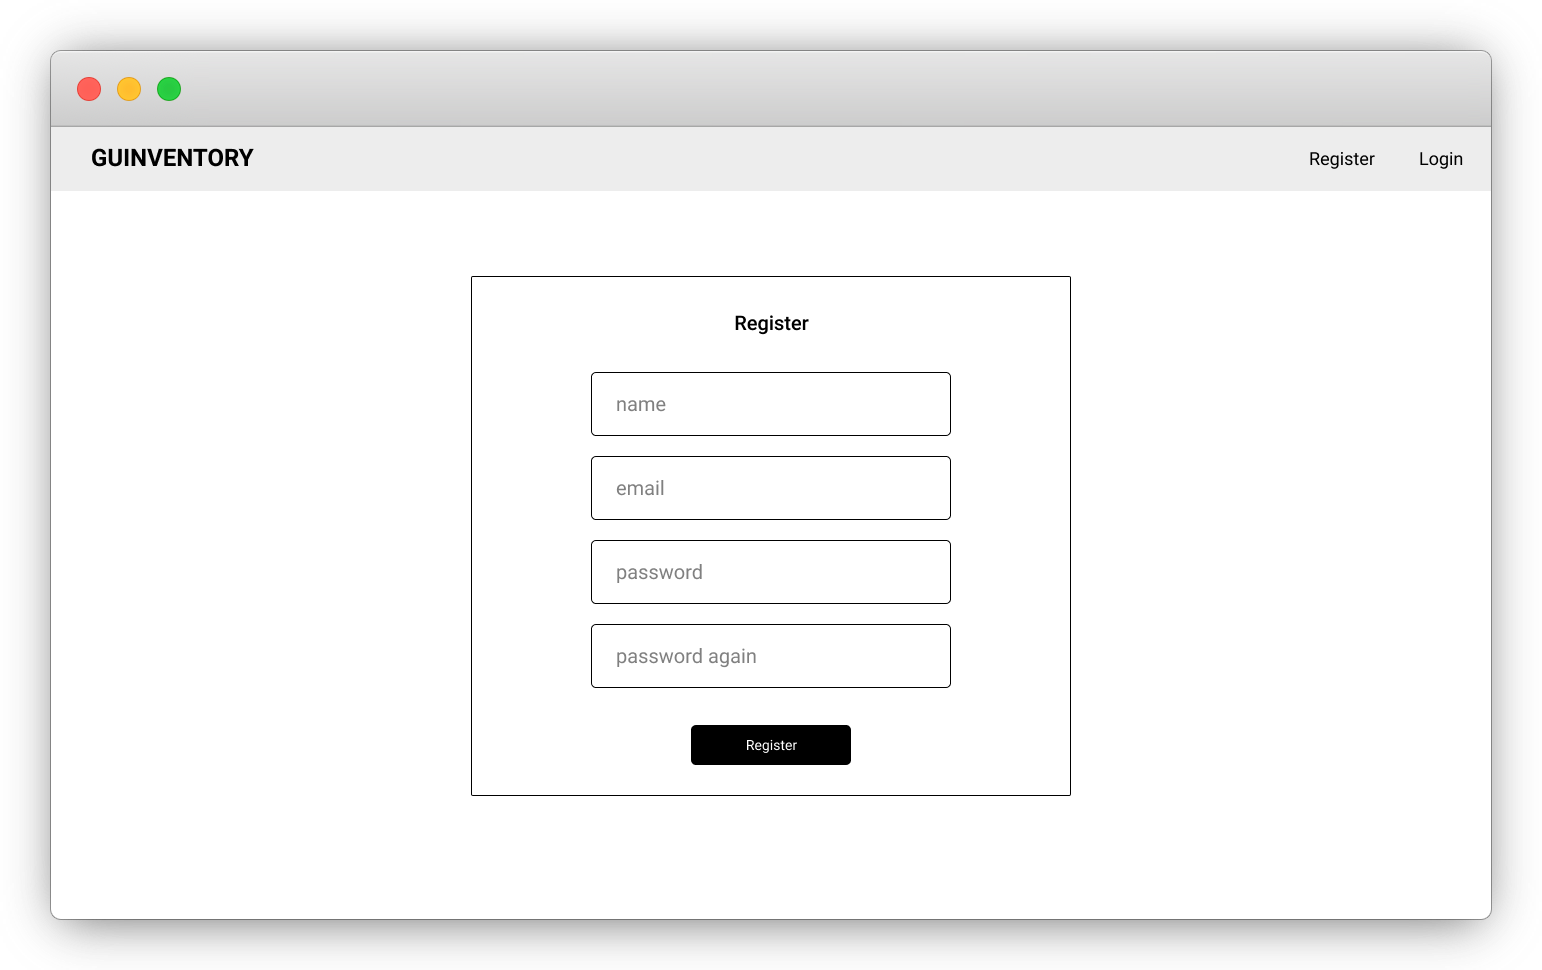
\includegraphics[width=150mm, keepaspectratio]{figures/wireframes/frame_registration.png}
  \caption{Regisztráció wireframe}
  \label{fig:RegistrationWireframe}
\end{figure}


\section{Raktár nézet}
A raktár oldalán (\refstruc{fig:WarehouseWireframe}) láthatunk egy térképes nézetet és egy listát is a tárololókról. 
A térképes nézeten a kurzort a tároló fülé mozgatva megjelnítjük annak nevét a könnyebb azonosítás érdeképben.

Ezen felül a navigációs bárban láthatjük az éppen kiválasztot raktárat, ahol egy legördülő menü segítségével azonnal választhatunk másik raktárat is, amennyiben több raktárhoz is van hozzáférésünk.
A raktár választó mellett megjelenítünk egy gombot, amellyel új tárolót hozhatunk létre.
\begin{figure}[!ht]
  \centering
  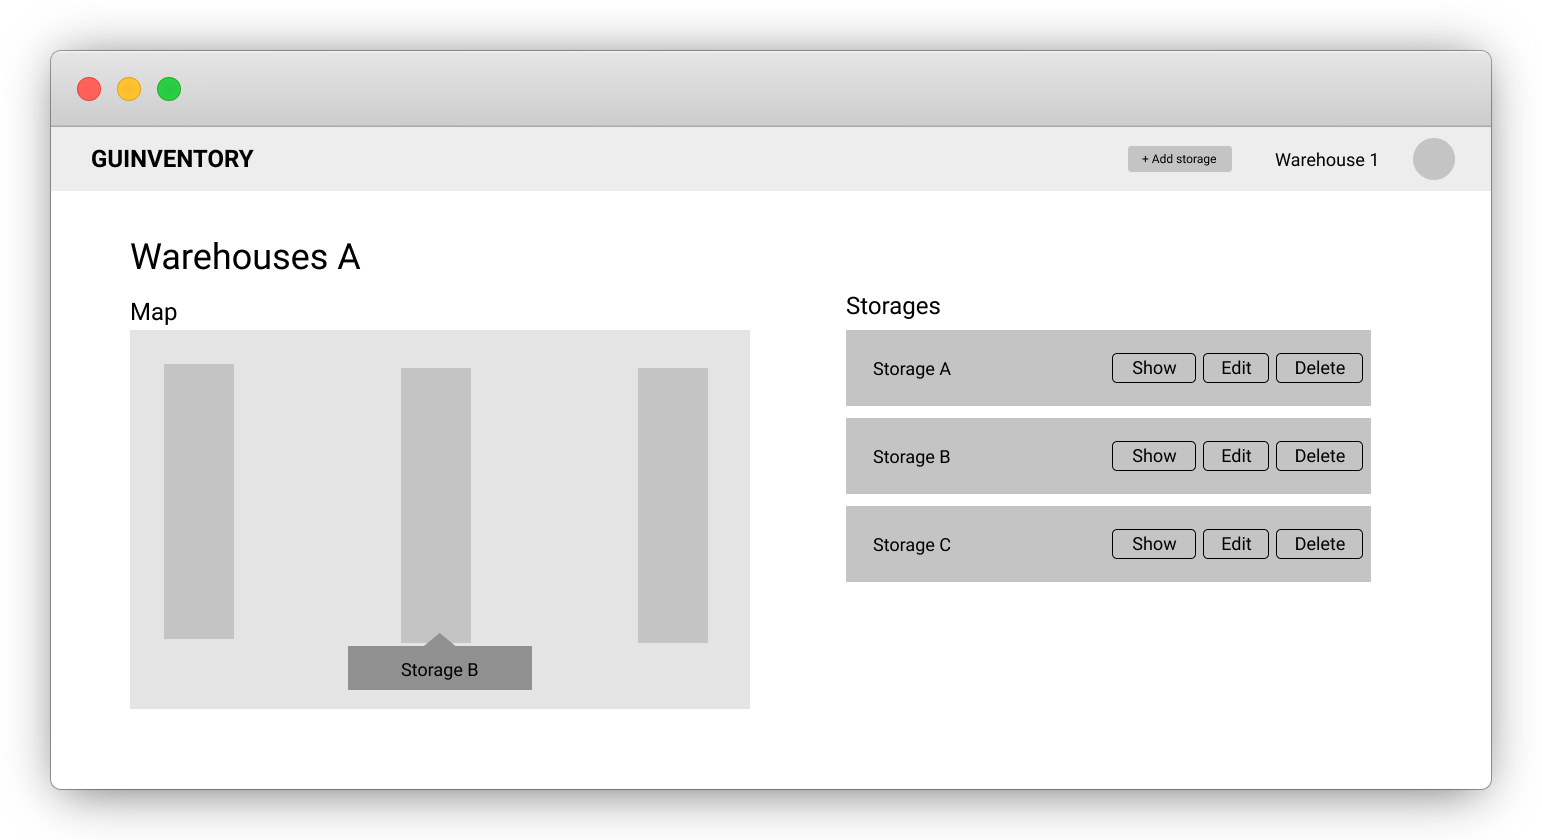
\includegraphics[width=150mm, keepaspectratio]{figures/wireframes/frame_warehouse.png}
  \caption{Raktár wireframe}
  \label{fig:WarehouseWireframe}
\end{figure}

\section{Tároló nézet}
A tároló nézete (\refstruc{fig:StorageWireframe}) nagyban hasonlít a raktáréhoz, azonban itt kiegészítésképt a térkép felett megjelenítünk egy másik tárolót.
Ez a feladatspecifikációban megkövetelt tárolók közötti eszköz mozgatását teszi lehetővé.

A navigációs bárban itt is megjelenítjük a raktár választó gombot, azonban a tároló létrehozása helyett, itt az eszköz felvétele gombot találhatjuk.

\begin{figure}[!ht]
  \centering
  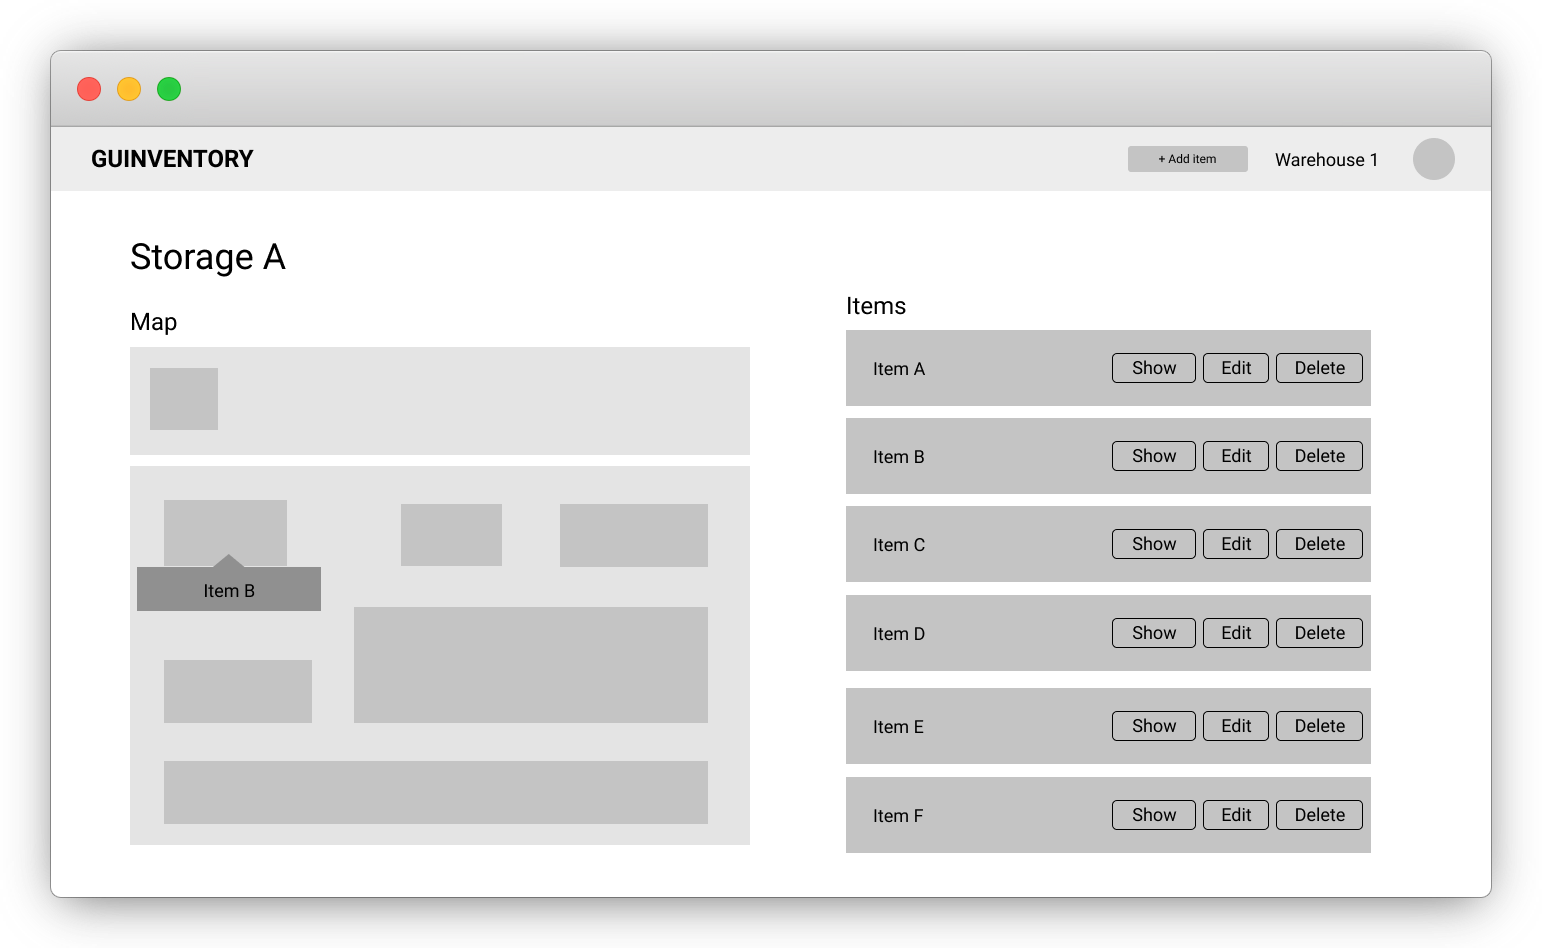
\includegraphics[width=150mm, keepaspectratio]{figures/wireframes/frame_storage.png}
  \caption{Tároló wireframe}
  \label{fig:StorageWireframe}
\end{figure}
  